% ==============================================================================
% PAGE 30: 12) WOODEN BASE, PVC PIPE & VARIOUS TYPES OF NUT (Numbered Page 22)
% ==============================================================================
\subsubsection*{12) WOODEN BASE, PVC PIPE \& VARIOUS TYPES OF NUT}

\begin{center}
  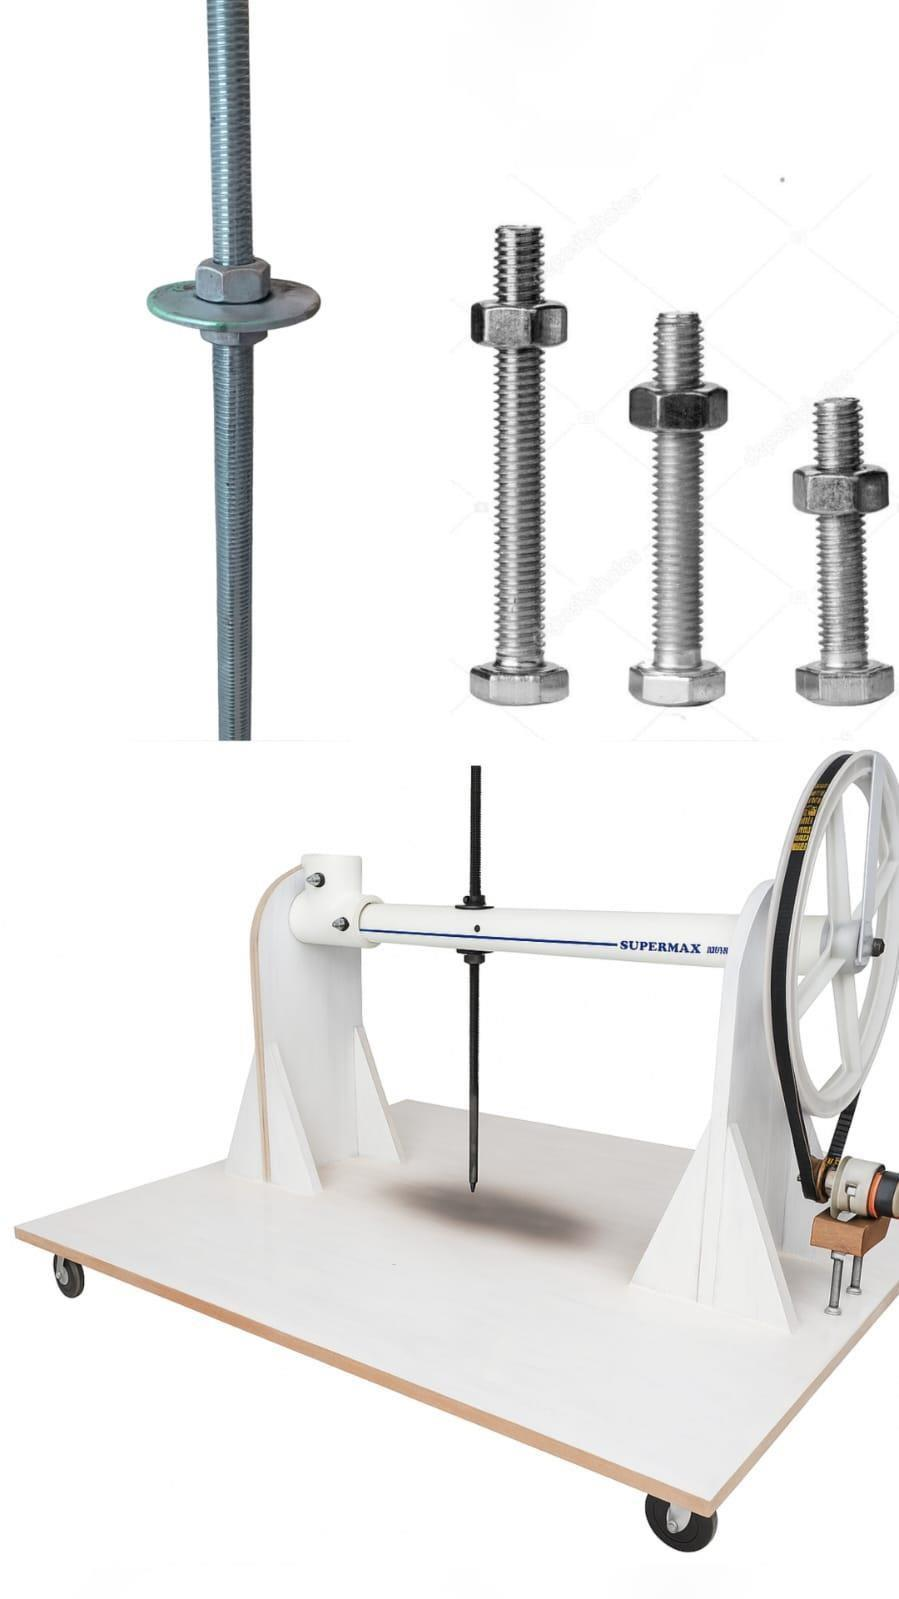
\includegraphics[width=75mm]{figures/fig14_wooden_base_assembly.jpg}
\end{center}

\noindent
\begin{spacing}{1.2}
{\fontsize{10.2}{14.5}\selectfont
The stud rod is a fully threaded rod that provides adjustable connections using nuts and washers at both ends. Different types of nuts and bolts are used to fix and support various parts of the assembly securely. The PVC pipe acts as the main shaft, on which the pulley is mounted. This shaft transmits rotational motion from the motor to the parabolic dish, allowing smooth and stable operation.\\[3mm]
The motor and pulley arrangement are connected through a belt drive, which transfers torque efficiently to the PVC shaft. The base platform of size 60 $\times$ 60 cm is made from a wooden sheet, providing a strong and stable foundation for the entire setup. This design ensures that all components remain firmly in place during the operation and allows precise and balanced rotation of the parabolic dish for tracking or positioning purposes.
}
\end{spacing}
\clearpage
